\newpage
\section{Méthodologie du développement}
\subsection{Introduction}
\noindent
Toute réalisation du projet doit être précédée d’une méthode de développement et un langage d’analyse et de conception, qui ont pour but de permettre de définir les étapes préliminaires de d´eveloppement d’un projet afin de rendre ce développement plus facile et plus flexible aux besoins et d’éviter tout retard au niveau du délai. En se basant sur ce constat, et pour une organisation adéquate de développement du projet et pour faciliter et accélérer la transformation
des besoins des utilisateurs en un systéme logiciel, nous avons opté pour l’approche SCRUM comme processus de travail et UML comme langage de modélisation.

\subsection{Méthode Adoptée: SCRUM}
\noindent
{\small\textbf{\textit{a. Définition}}}\mbox{}\\
Le principe de la méthode agile SCRUM est de concentrer l'équipe de développement sur un ensemble de fonctionnalités à réaliser de façon itérative, dans des itérations d'une durée de deux à quatre semaines, appelées des Sprints. Chaque Sprint commence par une estimation suivie d'une planification opérationnelle et se termine par une démonstration de ce qui a été achevé.

\noindent
{\small\textbf{\textit{b. Pourquoi SCRUM?}}}\mbox{}\\
Avant, le client ne voyait pas l'évolution du travail et n'était pratiquement pas impliqué pendant l'exécution de son projet. En effet, il ne pouvait pas commencer à faire des tests avant que tout soit presque fini. Par contre en Scrum, le client est de plus en plus impliqué dans le processus où il sera appelé à valider les livrables. À chaque livrable, les fonctionnalités sont en amélioration continue et le client voit régulièrement l'évolution des travaux et peut intervenir pour ajuster ses besoins.

\noindent
C'est pourquoi, Scrum vise essentiellement à optimiser la prévisibilité d'un projet et à mieux contrôler les risques.


\noindent
{\small\textbf{\textit{c. Les Artefacts SCRUM:}}}\mbox{} \\
Les artefacts Scrum sont des éléments du cadre Scrum qui matérialisent le travail à faire ou la valeur à apporter, ainsi que l'avancement du travail réalisé par l'équipe. Il existe trois artefacts tels que décrit dans le guide :

\begin{itemize}
  \item \small\textbf{Le Backlog Produit}, ou (\textit{Product backlog} en anglais) : est une liste ordonnée et en constante évolution du travail à réaliser afin d'améliorer le produit.
  
  \item \small\textbf{Le Backlog Sprint}, ou (\textit{Sprint backlog} en anglais) : Le Sprint backlog est une liste contenant les spécifications techniques pour les tâches devant être accomplis par l'équipe de développement au cours d'une période donnée (sprint).
  
  \item \small\textbf{Livraision}, ou (\textit{Delivery} en anglais) : la version du produit livrée aux parties prenantes après chaque sprint.
\end{itemize}

La Figure~\ref{fig:scrum} représente méthodologie SCRUM.

\begin{figure}[H]
\centering
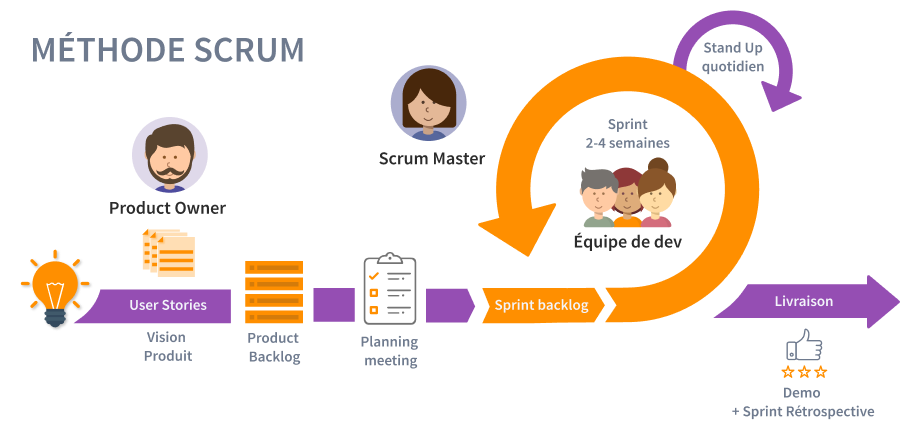
\includegraphics[width=1\textwidth]{logos/scrum.png}
\caption{Présentation du processus SCRUM}
\label{fig:scrum}
\end{figure}

\newpage
\noindent
{\small\textbf{\textit{d. Les rôles de la méthode Scrum :}}}\mbox{} \\
L'adoption de Scrum requiert la mise en place de 3 rôles spécifiques. Il s'agit du: Product owner, de l'équipe de développement et du Scrum master.

\begin{itemize}
  \item \small\textbf{Product Owner: } Le product owner (PO) représente le client ou l'utilisateur final. Son rôle est de veiller à ce que le produit soit conforme aux attentes du client que ce soit en terme de qualité ou de valeur ajoutée.
  
  \item \small\textbf{Scrum Master: } Il est le leader de l'équipe, il s'assure que le scrum est correctement appliqué et respecté et enlève les obstacles qui peuvent perturber l'avancement des travaux.
  
  \item \small\textbf{l'équipe de Développement: } L'équipe de développement est chargée de la mise en œuvre des solutions techniques et de la réalisation des développements requis.
\end{itemize}

\subsection{Le Langage UML}
\noindent
Après le choix de la méthodologie de développement, nous avons besoin d’un langage de modélisation unifié pour la modélisation de notre projet. Pour concevoir notre système, nous avons choisi UML (Unified Modeling Language) comme un langage de modélisation qui couvre les différentes vues du projet. Notre choix s’est basé sur les points forts de ce langage notamment sa standardisation et les divers diagrammes qu’il propose.

\section{Conclusion}
\noindent
Dans ce chapitre, nous avons présenté le cadre général de notre projet en déterminant la problématique et en proposant une solution. Nous avons dévoilé la méthodologie de développement et la méthode de conception qui seront utilisées dans les prochains chapitres de ce rapport et nous avons argumenté notre choix.

\newpage